\documentclass[crop,tikz]{standalone}

\usetikzlibrary{decorations.markings}

\tikzset{>=latex}
\colorlet{green}{black!40!green}

\tikzset{%
  >=latex, % default arrow style
  ->-/.style={postaction={decorate},decoration={%
      markings,mark=at position #1 with {\arrow{>}}%
    }%
  },%
  ->-/.default=.5,%
  -<-/.style={postaction={decorate},decoration={%
      markings,mark=at position #1 with {\arrowreversed{>}}%
    }%
  },%
  -<-/.default=.5%
}

% eye
\newcommand{\eye}[4]{% size, x, y, rotation
  \draw[rotate around={#4:(#2,#3)}] (#2,#3) -- ++(-.5*55:#1) (#2,#3) -- ++(.5*55:#1);
  \draw (#2,#3) ++(#4+55:.75*#1) arc (#4+55:#4-55:.75*#1);
  % iris
  \draw[fill=gray] (#2,#3) ++(#4+55/3:.75*#1) arc (#4+180-55:#4+180+55:.28*#1);
  % pupil, a filled arc 
  \draw[fill=black] (#2,#3) ++(#4+55/3:.75*#1) arc (#4+55/3:#4-55/3:.75*#1);
}

\begin{document}
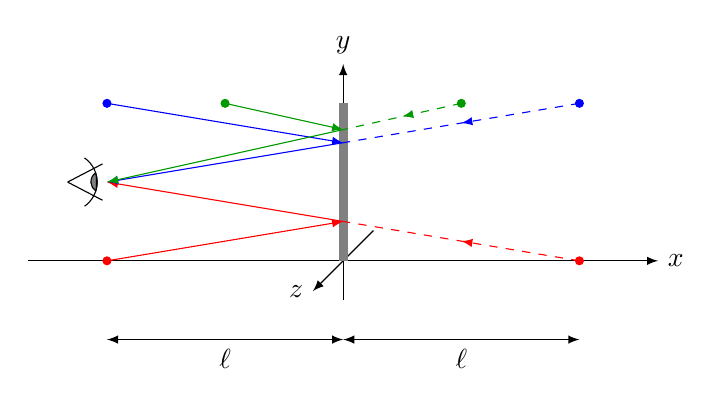
\begin{tikzpicture}
  % axis
  \draw[->] (-4,0)   -- (4,0)   node[right] {$x$};
  \draw[->] (0,-0.5) -- (0,2.5) node[above] {$y$};
  \draw[->] (0,0,-1) -- (0,0,1) node[left]  {$z$};
  % mirror
  \draw[fill,gray] (-0.05,0) rectangle (0.05,2);
  % coordinates
  \coordinate (eye) at (-3,1);
  \coordinate (r)   at (-3,0);
  \coordinate (rs)  at (0,0.5);
  \coordinate (rp)  at (3,0);
  \coordinate (b)   at (-3,2);
  \coordinate (bs)  at (0,1.5);
  \coordinate (bp)  at (3,2);
  \coordinate (c)   at (-1.5,2);
  \coordinate (cs)  at (0,5/3);
  \coordinate (cp)  at (1.5,2);
  \draw[fill,red ]  (r)  circle (0.05);
  \draw[fill,red ]  (rp) circle (0.05);
  \draw[fill,blue]  (b)  circle (0.05);
  \draw[fill,blue]  (bp) circle (0.05);
  \draw[fill,green] (c)  circle (0.05);
  \draw[fill,green] (cp) circle (0.05);
  % Strahlen
  \draw[->,red] (r) -- (rs);
  \draw[->,red] (rs) -- (eye);
  \draw[->-,red,dashed] (rp) -- (rs);
  \draw[->,blue] (b) -- (bs);
  \draw[->,blue] (bs) -- (eye);
  \draw[->-,blue,dashed] (bp) -- (bs);
  \draw[->,green] (c) -- (cs);
  \draw[->,green] (cs) -- (eye);
  \draw[->-,green,dashed] (cp) -- (cs);
  % eye
  \eye{0.5}{-3.5}{1}{0};
  % distance
  \draw[<->] (+3,-1) -- node[below] {$\ell$} (0,-1);
  \draw[<->] (-3,-1) -- node[below] {$\ell$} (0,-1);
\end{tikzpicture}
\end{document}
